\chapter{Homotopy Transfer}
\label{app:homotopy-transfer}
\index{homotopy transfer theorem|textbf}

The homotopy transfer theorem is one of the most powerful tools in homological 
algebra, allowing algebraic structures to be transported along quasi-isomorphisms 
at the cost of introducing higher operations. For chiral algebras, this provides 
the mechanism for constructing minimal models and understanding the relationship 
between different presentations of the same homotopy type.

\section{The Homotopy Transfer Theorem}
\label{sec:htt}

\begin{theorem}[Homotopy Transfer Theorem; \ClaimStatusProvedElsewhere]
\label{thm:htt}
Let $(V, d_V)$ and $(W, d_W)$ be chain complexes with:
\begin{enumerate}[label=(\roman*)]
\item A chain map $p: V \to W$ (projection).
\item A chain map $\iota: W \to V$ (inclusion).
\item A chain homotopy $h: V \to V[-1]$ satisfying $\id_V - \iota p = d_V h + h d_V$.
\item The \textbf{side conditions}: $p \iota = \id_W$, $h \iota = 0$, $p h = 0$, $h^2 = 0$.
\end{enumerate}
Such data is called a \textbf{strong deformation retract} (SDR).

If $V$ carries a $\cP_\infty$-algebra structure (for $\cP$ a Koszul operad), 
then $W$ inherits a $\cP_\infty$-algebra structure such that $p$ and $\iota$ 
extend to $\infty$-quasi-isomorphisms of $\cP_\infty$-algebras.
\end{theorem}

\begin{proof}[Proof sketch]
The transferred structure on $W$ is constructed via the \textbf{tensor trick}. 
For an $\Ainf$-algebra structure on $V$ with operations $m_n: V^{\otimes n} \to V$, 
the transferred operations $\tilde{m}_n: W^{\otimes n} \to W$ are:
\[
\tilde{m}_n := p \circ T_n \circ \iota^{\otimes n}
\]
where $T_n: V^{\otimes n} \to V$ sums over all ways of inserting $h$ and $m_k$ 
in trees. Explicitly:
\begin{align*}
\tilde{m}_1 &= p \, d_V \, \iota = d_W \\
\tilde{m}_2 &= p \, m_2 \, \iota^{\otimes 2} \\
\tilde{m}_3 &= p \, m_3 \, \iota^{\otimes 3} + p \, m_2 (h m_2 \otimes \id) \, \iota^{\otimes 3} 
              + p \, m_2 (\id \otimes h m_2) \, \iota^{\otimes 3}
\end{align*}
and so on. The $\Ainf$-relations for $\{\tilde{m}_n\}$ follow from those for 
$\{m_n\}$ and the SDR properties.
\end{proof}

\begin{definition}[Strong Deformation Retract Data]
\label{def:sdr}
\index{strong deformation retract|textbf}
\index{SDR|see{strong deformation retract}}
A \textbf{strong deformation retract} (SDR) from $V$ to $W$ is a tuple 
$(V, W, p, \iota, h)$ satisfying the conditions of Theorem~\ref{thm:htt}. 
We denote this by:
\[
\begin{tikzcd}[column sep=large]
(V, d_V) \arrow[r, shift left, "p"] & (W, d_W) \arrow[l, shift left, "\iota"]
\end{tikzcd}
\quad h: V \to V[-1], \quad \id - \iota p = dh + hd.
\]
The diagram commutes up to homotopy $h$.
\end{definition}

\begin{lemma}[Existence of SDR; \ClaimStatusProvedHere]
\label{lem:sdr-existence}
If $V \xrightarrow{\sim} W$ is a quasi-isomorphism of chain complexes over a 
field $k$, then:
\begin{enumerate}[label=(\roman*)]
\item There exists an SDR from $V$ to $H_*(V) = H_*(W)$.
\item If $V$ and $W$ are both semi-free (or projective as graded modules), 
there exists an SDR between them.
\end{enumerate}
\end{lemma}

\begin{proof}
(i) Choose a splitting $V = H_*(V) \oplus B \oplus C$ where $d: C \xrightarrow{\sim} B$ 
is an isomorphism (decomposition into homology, boundaries, and ``extra'' cycles 
that become boundaries). Define:
\[
\iota: H_*(V) \hookrightarrow V, \quad p: V \twoheadrightarrow H_*(V), \quad 
h: V \to V[-1]
\]
where $h$ sends $B$ to $C$ via the inverse of $d|_C$, and is zero on $H_*(V) \oplus C$.
One verifies: $p \circ \iota = \mathrm{id}_{H_*(V)}$ (by definition), $\iota \circ p - \mathrm{id}_V = d \circ h + h \circ d$ (since $h$ inverts $d$ on the acyclic summand $B \oplus C$ and vanishes on $H_*(V)$), and $h^2 = h \circ \iota = p \circ h = 0$ (the annihilation conditions hold because $h$ maps $B \to C$, which is disjoint from its domain of support).

(ii) The Comparison Theorem for projective resolutions provides the maps; 
standard homological algebra constructs the homotopy.
\end{proof}


\section{Explicit Formulas for Transferred Structures}
\label{sec:transfer-formulas}

\begin{construction}[Transferred $\Ainf$-Structure]
\label{constr:transfer-ainf}
Let $(A, \{m_n\})$ be an $\Ainf$-algebra and $(A, H, p, \iota, h)$ an SDR to 
the homology $H = H_*(A)$. The transferred $\Ainf$-structure $\{\tilde{m}_n\}$ 
on $H$ is given by:

\textbf{$\tilde{m}_1 = 0$}: The differential on homology vanishes.

\textbf{$\tilde{m}_2$}: The induced product:
\[
\tilde{m}_2(a, b) = p \, m_2(\iota(a), \iota(b)).
\]

\textbf{$\tilde{m}_3$}: The \textbf{Massey product} or $\Ainf$-associator:
\begin{align*}
\tilde{m}_3(a, b, c) &= p \, m_3(\iota(a), \iota(b), \iota(c)) \\
&\quad + p \, m_2(h \, m_2(\iota(a), \iota(b)), \iota(c)) \\
&\quad + (-1)^{|a|}\, p \, m_2(\iota(a), h \, m_2(\iota(b), \iota(c))).
\end{align*}
The sign $(-1)^{|a|}$ arises from commuting the homotopy $h$ (degree $-1$) past $\iota(a)$ (degree $|a|$) via the Koszul sign rule.

\textbf{$\tilde{m}_n$} (general): Sum over planar rooted trees $T$ with $n$ 
leaves:
\[
\tilde{m}_n = \sum_{T \in \mathrm{PRT}_n} p \, T(m_\bullet, h, \iota)
\]
where $T(m_\bullet, h, \iota)$ places $\iota$ at leaves, $m_k$ at vertices of 
valence $k$, and $h$ on internal edges.
\end{construction}

\begin{theorem}[Tree Formula for Transferred Operations; \ClaimStatusProvedElsewhere]
\label{thm:tree-formula}
\index{tree formula!for transfer}
The transferred $n$-ary operation is:
\[
\tilde{m}_n = \sum_{T \in \mathrm{PRT}_n} \epsilon(T) \cdot p \circ \prod_{v \in V(T)} 
m_{|v|} \circ \prod_{e \in E_{\mathrm{int}}(T)} h \circ \iota^{\otimes n}
\]
where:
\begin{enumerate}[label=(\roman*)]
\item $\mathrm{PRT}_n$ is the set of planar rooted trees with $n$ leaves.
\item $V(T)$ is the set of internal vertices; $|v|$ is the valence of $v$.
\item $E_{\mathrm{int}}(T)$ is the set of internal edges.
\item $\epsilon(T) \in \{\pm 1\}$ is a sign determined by the Koszul rule.
\end{enumerate}
\end{theorem}

\begin{remark}[Tree-Level Only]\label{rem:tree-level}
A fundamental feature of the homotopy transfer theorem is that \emph{only tree-level graphs contribute}: the sum in Theorem~\ref{thm:tree-formula} runs over trees (acyclic connected graphs), never over graphs with loops.  This is because the side condition $h^2 = 0$ ensures that any graph with a cycle (which would route through $h$ at least twice on a closed path) vanishes.  In the chiral algebra setting, this means the transferred operations are algebraic (finite sums), not analytic, and no renormalization issues arise.
\end{remark}

\begin{example}[Trees for $\tilde{m}_4$]
\label{ex:trees-m4}
The trees contributing to $\tilde{m}_4$ are:

\begin{enumerate}[label=(\arabic*)]
\item One vertex of valence 4:
\[
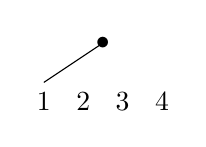
\begin{tikzpicture}[scale=0.5]
\node at (0,1) {$\bullet$};
\draw (0,1) -- (-1.5,0) (-0.5,0) (0.5,0) (1.5,0);
\draw (-1.5,0) node[below] {$1$};
\draw (-0.5,0) node[below] {$2$};
\draw (0.5,0) node[below] {$3$};
\draw (1.5,0) node[below] {$4$};
\end{tikzpicture}
\quad \leadsto \quad p \, m_4 \, \iota^{\otimes 4}
\]

\item One vertex of valence 3, one of valence 2 (5 configurations --- the binary vertex can be a child of the ternary in 3 ways, or the ternary can be a child of the binary in 2 ways):
\[
p \, m_3(h \, m_2 \otimes \id \otimes \id) \, \iota^{\otimes 4}, \quad
p \, m_2(h \, m_3 \otimes \id) \, \iota^{\otimes 4}, \quad \ldots
\]

\item Three vertices of valence 2 (5 configurations --- the Catalan number $C_3 = 5$ binary trees with 4 leaves).
\end{enumerate}
Total: $1 + 5 + 5 = 11$ planar rooted trees with 4 leaves and all internal vertices of arity $\geq 2$.
\end{example}

\begin{proposition}[Sign Computation; \ClaimStatusProvedElsewhere]
\label{prop:transfer-signs}
The sign $\epsilon(T)$ in the tree formula is:
\[
\epsilon(T) = (-1)^{\sum_{e \in E_{\mathrm{int}}(T)} (|e|_{\mathrm{left}} + 1)}
\]
where $|e|_{\mathrm{left}}$ is the sum of degrees of inputs to the left of 
edge $e$ (counting the edge as separating left from right at its source vertex).
\end{proposition}


\section{Applications to Minimal Models}
\label{sec:minimal-models}

\begin{definition}[Minimal Model]
\label{def:minimal-model}
\index{minimal model|textbf}
A \textbf{minimal model} of a dg-algebra $A$ is an $\Ainf$-algebra $M$ with:
\begin{enumerate}[label=(\roman*)]
\item $M$ has zero differential: $m_1 = 0$.
\item There is an $\Ainf$-quasi-isomorphism $M \xrightarrow{\sim} A$.
\end{enumerate}
A minimal model is unique up to $\Ainf$-isomorphism.
\end{definition}

\begin{theorem}[Existence of Minimal Models; \ClaimStatusProvedElsewhere]
\label{thm:minimal-model-existence}
Every $\Ainf$-algebra over a field admits a minimal model. Explicitly, if 
$A$ is an $\Ainf$-algebra:
\begin{enumerate}[label=(\roman*)]
\item Take $M = H_*(A)$ as a graded vector space.
\item Choose an SDR $(A, H_*(A), p, \iota, h)$.
\item Apply the homotopy transfer theorem to get $\{m_n\}_{n \geq 2}$ on $M$.
\item The resulting $(M, 0, m_2, m_3, \ldots)$ is the minimal model.
\end{enumerate}
\end{theorem}

\begin{corollary}[Formality; \ClaimStatusProvedElsewhere]
\label{cor:formality}
An $\Ainf$-algebra $A$ is \textbf{formal} if its minimal model has $m_n = 0$
for all $n \geq 3$, i.e., the minimal model is a graded associative
algebra with trivial differential and no higher operations.

Equivalently, $A$ is formal if $A \simeq H_*(A)$ as $\Ainf$-algebras, where 
$H_*(A)$ has the trivial $\Ainf$-structure from its product.
\end{corollary}

\begin{example}[Minimal Model of de Rham Complex]
\label{ex:minimal-derham}
For $X = S^1$ (circle), the de Rham complex is:
\[
(\Omega^*(S^1), d) = (k \xrightarrow{0} k, \quad 1 \mapsto 0, \quad d\theta \mapsto 0)
\]
with cohomology $H^* = k \oplus k[-1]$.

The minimal model has:
\begin{enumerate}[label=(\roman*)]
\item $M = k \cdot 1 \oplus k \cdot x$ with $|1| = 0$, $|x| = 1$.
\item $m_2(1, 1) = 1$, $m_2(1, x) = m_2(x, 1) = x$, $m_2(x, x) = 0$.
\item $m_n = 0$ for $n \geq 3$ (the circle is formal).
\end{enumerate}
\end{example}

\begin{application}[Minimal Model for Chiral Algebras]
\label{app:minimal-chiral}
For a chiral algebra $\cA$, the homotopy transfer theorem provides:
\begin{enumerate}[label=(\roman*)]
\item A minimal $\Ainf$-chiral structure on $H^{\mathrm{ch}}_*(\cA)$.
\item The higher operations $\{m_n\}_{n \geq 3}$ encode obstructions to formality.
\item For Koszul chiral algebras, the minimal model often simplifies dramatically.
\end{enumerate}

For the Heisenberg algebra $\cH$:
\[
H^{\mathrm{ch}}_*(\cH) = k
\]
is 1-dimensional (Koszul), and the minimal model is the ground field with 
trivial structure.
\end{application}

\begin{theorem}[Homotopy Transfer for Operadic Algebras; \ClaimStatusProvedElsewhere]
\label{thm:htt-operadic}
Let $\cP$ be a Koszul operad and $(A, W, p, \iota, h)$ an SDR with $A$ a 
$\cP$-algebra. The transferred $\cP_\infty$-structure on $W$ satisfies:
\begin{enumerate}[label=(\roman*)]
\item The $\cP_\infty$-relations hold on the nose (not just up to homotopy).
\item The maps $\iota$ and $p$ extend to $\infty$-morphisms.
\item If $A$ is already $\cP_\infty$ (not just $\cP$), the transfer still works.
\end{enumerate}
\end{theorem}


\section{Extended Formulas and Computational Techniques}
\label{sec:extended-htt}

We provide extended formulas for homotopy transfer that are essential for 
explicit computations in chiral Koszul duality.

\begin{construction}[Homotopy Transfer for $\Linf$-Algebras]
\label{constr:htt-linf}
Let $(\fg, \{l_n\})$ be an $\Linf$-algebra and $(\fg, H, p, \iota, h)$ an SDR. 
The transferred $\Linf$-structure on $H$ has brackets:

\textbf{$\tilde{l}_1 = 0$}: Differential vanishes on homology.

\textbf{$\tilde{l}_2$}: The induced Lie bracket:
\[
\tilde{l}_2(a, b) = p \, l_2(\iota(a), \iota(b)).
\]

\textbf{$\tilde{l}_3$}: The \textbf{Massey--Lie bracket} or Jacobiator:
\begin{align*}
\tilde{l}_3(a, b, c) &= p \, l_3(\iota(a), \iota(b), \iota(c)) \\
&\quad + p \, l_2(h \, l_2(\iota(a), \iota(b)), \iota(c)) \\
&\quad + (-1)^{|b||c|} \, p \, l_2(h \, l_2(\iota(a), \iota(c)), \iota(b)) \\
&\quad + (-1)^{|a|(|b|+|c|)} \, p \, l_2(h \, l_2(\iota(b), \iota(c)), \iota(a)).
\end{align*}

The signs arise from the graded antisymmetry of the Lie bracket.
\end{construction}

\begin{proposition}[$\Linf$-Relations for Transferred Structure; \ClaimStatusProvedElsewhere]
\label{prop:linf-relations}
The transferred brackets $\{\tilde{l}_n\}$ satisfy the $\Linf$-relations:
\[
\sum_{i+j = n+1} \sum_{\sigma \in \mathrm{Sh}(i, n-i)} \epsilon(\sigma) 
\tilde{l}_j(\tilde{l}_i(x_{\sigma(1)}, \ldots, x_{\sigma(i)}), x_{\sigma(i+1)}, \ldots, x_{\sigma(n)}) = 0
\]
where $\mathrm{Sh}(i, n-i)$ denotes $(i, n-i)$-unshuffles and $\epsilon(\sigma)$ 
is the Koszul sign.
\end{proposition}

\begin{computation}[Explicit $\tilde{l}_4$ Formula]
\label{comp:l4-formula}
The 4-ary transferred bracket is:
\begin{align*}
\tilde{l}_4(a, b, c, d) &= p \, l_4(\iota a, \iota b, \iota c, \iota d) \\
&\quad + \sum_{\sigma \in S_4} \epsilon_\sigma \, p \, l_3(h l_2(\iota x_{\sigma_1}, \iota x_{\sigma_2}), \iota x_{\sigma_3}, \iota x_{\sigma_4}) \\
&\quad + \sum_{\text{pairings}} \epsilon \, p \, l_2(h l_2(\iota a, \iota b), h l_2(\iota c, \iota d)) \\
&\quad + \sum_{\sigma} \epsilon_\sigma \, p \, l_2(h l_3(\iota x_{\sigma_1}, \iota x_{\sigma_2}, \iota x_{\sigma_3}), \iota x_{\sigma_4}) \\
&\quad + \text{(trees with two internal edges)}
\end{align*}
The full formula involves 25 terms corresponding to trees with 4 leaves.
\end{computation}

\begin{theorem}[Uniqueness of Minimal $\Linf$-Model; \ClaimStatusProvedElsewhere]
\label{thm:linf-minimal-unique}
If $(\fg, \{l_n\})$ is an $\Linf$-algebra over a field:
\begin{enumerate}[label=(\roman*)]
\item A minimal $\Linf$-model $(H, \{\tilde{l}_n\})$ exists with $\tilde{l}_1 = 0$.
\item Any two minimal $\Linf$-models are $\Linf$-isomorphic.
\item The isomorphism is unique up to $\Linf$-homotopy.
\end{enumerate}
\end{theorem}

\begin{construction}[Homotopy Transfer for Coalgebras]
\label{constr:htt-coalg}
For a dg-coalgebra $(C, \Delta, d)$ and SDR $(C, H, p, \iota, h)$, the transferred 
$\Ainf$-coalgebra structure on $H$ has coproducts:

\textbf{$\tilde{\Delta}_1 = 0$}: No differential on homology.

\textbf{$\tilde{\Delta}_2$}: The induced coproduct:
\[
\tilde{\Delta}_2(c) = (p \otimes p) \Delta(\iota(c)).
\]

\textbf{$\tilde{\Delta}_n$ for $n \geq 3$}: Higher coproducts from trees:
\[
\tilde{\Delta}_n = \sum_{T \in \mathrm{Trees}_n} \epsilon(T) \cdot (p^{\otimes n}) \circ T(\Delta, h) \circ \iota
\]
where trees now have edges ``pointing down'' (toward outputs) rather than up.
\end{construction}

\begin{example}[Transfer for Symmetric Coalgebra]
\label{ex:transfer-sym-coalg}
Let $C = S^c(V)$ be the symmetric coalgebra on a chain complex $(V, d_V)$. 
The coproduct is deconcatenation:
\[
\Delta(v_1 \cdots v_n) = \sum_{I \sqcup J = [n]} v_I \otimes v_J
\]
where $v_I = \prod_{i \in I} v_i$ (in order).

If $V \xrightarrow{p} H_*(V) =: W$ is a deformation retract:
\begin{enumerate}[label=(\roman*)]
\item $\tilde{\Delta}_2$ on $S^c(W)$ is the standard deconcatenation (symmetric coalgebra).
\item $\tilde{\Delta}_3$ involves Massey products: corrections arise when $d_V$ is nontrivial.
\item If $V$ is formal (quasi-isomorphic to $H_*(V)$ with zero differential), then $\tilde{\Delta}_n = 0$ for $n \geq 3$.
\end{enumerate}
\end{example}


\section{Applications to Chiral Algebras}
\label{sec:htt-chiral}

The homotopy transfer theorem has specific applications to chiral algebra theory 
that deserve detailed exposition.

\begin{theorem}[Chiral Homotopy Transfer; \ClaimStatusProvedHere]
\label{thm:chiral-htt}
\index{$A_\infty$-structure!transferred}
Let $\cA$ be an $\Eone$-chiral algebra on a curve $X$ and suppose we have an 
SDR of the underlying D-module:
\[
(\cA, H, p, \iota, h) \quad \text{with } H = H^{\mathrm{ch}}_*(\cA).
\]
Then:
\begin{enumerate}[label=(\roman*)]
\item $H$ inherits an $\Ainf$-chiral algebra structure.
\item The higher operations $\{m_n^{\mathrm{ch}}\}_{n \geq 3}$ are ``Massey products'' 
for the chiral structure.
\item If $\cA$ is Koszul, then $m_n^{\mathrm{ch}} = 0$ for $n \geq 3$.
\end{enumerate}
\end{theorem}

\begin{proof}
We apply the general homotopy transfer theorem (Theorem~\ref{thm:htt}) to the $\Eone$-chiral operad.

\textbf{Step 1} (D-module compatibility): Since $\cA$ is a chiral algebra, it carries a $\cD_X$-module structure.  The SDR maps $(p, \iota, h)$ must be morphisms of $\cD_X$-modules (i.e., commute with the action of $\cD_X$).  This holds because chiral homology $H = H^{\mathrm{ch}}_*(\cA)$ is defined as a derived functor in the category of $\cD_X$-modules, so $p$ and $\iota$ are automatically $\cD_X$-linear, and $h$ can be chosen $\cD_X$-linearly by the splitting argument of Lemma~\ref{lem:sdr-existence}(i) applied within the $\cD_X$-module category (which is abelian with enough projectives over a smooth curve~$X$).

\textbf{Step 2} (Transferred binary operation): The transferred product is $\tilde{m}_2 = p \circ \mu^{\mathrm{ch}} \circ (\iota \otimes \iota)$, exactly as in Construction~\ref{constr:transfer-ainf}.  Since $\mu^{\mathrm{ch}}$ is a chiral product (defined via the $j_*j^*$ functor on $X \times X$), $\tilde{m}_2$ inherits $\cD_X$-linearity from Step~1.

\textbf{Step 3} (Higher operations via trees): The transferred operations $\tilde{m}_n^{\mathrm{ch}}$ for $n \geq 3$ are sums over planar rooted trees with $n$ leaves (as in Construction~\ref{constr:transfer-ainf}), where each internal edge contributes a factor of $h$ and each internal vertex contributes the chiral product $\mu^{\mathrm{ch}}$.  Since only tree-level graphs contribute (no loops; cf.\ Remark~\ref{rem:tree-level}), each $\tilde{m}_n^{\mathrm{ch}}$ is a finite sum.

\textbf{Step 4} ($\Ainf$-relations): The transferred operations $\{\tilde{m}_n^{\mathrm{ch}}\}$ satisfy the $\Ainf$-relations by the same algebraic argument as in the general theorem: the identity $\sum_{r+s+t=n}(-1)^{rs+t}\tilde{m}_{r+1+t}(\mathrm{id}^{\otimes r} \otimes \tilde{m}_s \otimes \mathrm{id}^{\otimes t}) = 0$ follows from substituting the tree formulas and using the $\Eone$-relations on $\cA$ together with the SDR identities $p\iota = \mathrm{id}$, $\mathrm{id} - \iota p = dh + hd$, $h^2 = 0$.

\textbf{Koszulness} (iii): If $\cA$ is Koszul, the bar complex $\bar{B}(\cA)$ has cohomology concentrated in a single bar degree. By the comparison theorem, the homotopy $h$ on $\bar{B}(\cA)$ vanishes in the relevant degrees, forcing all tree contributions with internal edges (i.e., $\tilde{m}_n^{\mathrm{ch}}$ for $n \geq 3$) to vanish.
\end{proof}

\begin{example}[Kac--Moody Minimal Model]
\label{ex:km-minimal}
For the affine Kac--Moody algebra $\hat{\fg}_k$ at level $k$ and a smooth projective curve $X$ of genus $g$:
\begin{enumerate}[label=(\roman*)]
\item The chiral homology $H^{\mathrm{ch}}_*(X, \hat{\fg}_k)$ depends on both $k$ and $g$.
\item At generic $k$ (irrational, or more precisely not a non-negative integer and not equal to $-h^\vee$): the higher chiral homology $H^{\mathrm{ch}}_i(X, \hat{\fg}_k) = 0$ for $i > 0$, while $H^{\mathrm{ch}}_0(X, \hat{\fg}_k)$ reduces to the space of conformal blocks, which is one-dimensional for the vacuum module \cite{BD04}.
\item At non-negative integral $k$: the chiral homology $H^{\mathrm{ch}}_*(X, \hat{\fg}_k)$ is related to spaces of conformal blocks for integrable representations, and the minimal model encodes this representation theory.
\item The transferred higher operations $m_n^{\mathrm{ch}}$ for $n \geq 3$
vanish by Koszulness of $\hat{\fg}_k$ (at non-critical level $k \neq -h^\vee$).
\end{enumerate}
\end{example}

\begin{proposition}[Transferred Structure and Bar Complex; \ClaimStatusProvedHere]
\label{prop:transfer-bar}
The homotopy transfer of chiral structures is compatible with the bar construction:
\[
\Bbar^{\mathrm{geom}}(H, \{\tilde{m}_n\}) \simeq \Bbar^{\mathrm{geom}}(\cA, \{m_n\})
\]
as geometric bar complexes. The quasi-isomorphism is induced by the SDR data.
\end{proposition}

\begin{proof}
The bar construction is functorial for $\infty$-morphisms. The SDR $(p, \iota, h)$ 
extends to an SDR on bar complexes:
\[
\Bbar(p), \Bbar(\iota), \Bbar(h): \Bbar(\cA) \rightleftarrows \Bbar(H).
\]
The compatibility with the geometric realization follows from the factorization 
property.
\end{proof}
